\documentclass[10pt,a4paper, margin=1in]{article}
\usepackage{fullpage}
\usepackage{amsfonts, amsmath, pifont}
\usepackage{amsthm}
\usepackage{cancel}
\usepackage{listings}
\usepackage{graphicx}
\usepackage{float}
\usepackage{mathrsfs}
\usepackage{tkz-euclide}
\usepackage{tikz}
\usepackage{pgfplots}
\usepackage[colorlinks=true, allcolors=black]{hyperref}

\pgfplotsset{compat=1.13}

\usepackage{geometry}
 \geometry{
 a4paper,
 total={210mm,297mm},
 left=10mm,
 right=10mm,
 top=10mm,
 bottom=10mm,
 }
 % Write both of your names here. Fill exxxxxxx with your ceng mail address.
 \author{
  Meyvecioğlu, Hasan Ege\\
  \texttt{e2449783@ceng.metu.edu.tr}
  \and
  Şanlı, Enes\\
  \texttt{e2375749@ceng.metu.edu.tr}
}

\title{CENG 384 - Signals and Systems for Computer Engineers \\
Spring 2023 \\
Homework 2}
\begin{document}
\maketitle



\noindent\rule{19cm}{1.2pt}

\begin{enumerate}

\item %write the solution of q1
    \begin{enumerate}
    % Write your solutions in the following items.
    \item %write the solution of q1a
The output of the adder is $y'(t)$, which is equal to $x(t) - 5*y(t)$.If we integrate $y'(t)$, we get the output signal $y(t)$. Hence:
\begin{equation}
    y'(t) = x(t) - 5y(t) \rightarrow y'(t) + 5y(t)= x(t) 
\end{equation}


    \item %write the solution of q1b
If $x(t) = (e^{-t} + e^{-3t})u(t) =e^{-t}u(t) + e^{-3t}u(t)$ and the system is initially at rest, then:
\begin{equation*}
    y(0) = y'(0) = 0
\end{equation*}
%%%%%%%%%%%%%%%%%%%%%%%%%%%%\begin{itemize}
    We can use Laplace transform to solve this ODE:
    \begin{equation*}
        \mathscr{L}\{y'(t)\} + 5 * \mathscr{L}\{y(t)\}=\mathscr{L}\{e^{-3t}*u(t)\} + \mathscr{L}\{e^{-t}*u(t)\} 
    \end{equation*}
    \begin{equation*}
        s*Y(s) - \cancel{y(0)} + 5 * Y(s) = \frac{1}{s+1} + \frac{1}{s+3}
    \end{equation*}
    \begin{equation*}
        (s+5)*Y(s) = \frac{1}{s+1} + \frac{1}{s+3}
    \end{equation*}
    \begin{equation*}
        Y(s) = \frac{2s+4}{(s+1)*(s+3)*(s+5)}
    \end{equation*}
    \begin{equation*}
        Y(s) = \frac{A}{s+1} + \frac{B}{s+3} + \frac{C}{s+5} 
    \end{equation*}
    \begin{equation*}
        As^2 + 8A*s + 15 A + Bs^2 + 6sB+5B+Cs^2+4Cs+3C = 2s+ 4
    \end{equation*}
    \begin{equation*}
        A + B + C = 0
    \end{equation*}
    \begin{equation*}
        8A + 6B + 4C = 2
    \end{equation*}
    \begin{equation*}
        15A + 5B + 3C = 4
    \end{equation*}
Those equations gives:
\begin{equation*}
    A = \frac{1}{4}, B = \frac{1}{2}, C = \frac{-3}{4}
\end{equation*}
Then,  $Y(s)$ becomes:
\begin{equation*}
    Y(s) = \frac{1}{4*s+1} + \frac{1}{2*(s+3)} + \frac{-3}{4*(s+5)}
\end{equation*}
Remember that we are trying to find the general solution $y(t)$ and we can find it by applying inverse Laplace transform on $Y(s)$:
\begin{equation*}
    \mathscr{L^{-1}}\{Y(s)\} = \mathscr{L^{-1}}\{\frac{1}{4*(s+1)}\} + \mathscr{L^{-1}}\{\frac{1}{2*(s+3)}\} +\mathscr{L^{-1}}\{\frac{-3}{4*(s+5)}\}
\end{equation*}
\begin{equation}
    y(t) = \frac{e^{-t}}{4} + \frac{e^{-3t}}{2} - \frac{3*e^{-5t}}{4}
\end{equation}
%%%%%%%%%%%%%%%%%%%%%%%%%%%%%%%%%%
    \end{enumerate}

\item %write the solution of q2  
	\begin{enumerate}
    % Write your solutions in the following items.
    \item %write the solution of q2a   
    \begin{equation*}
           x[n] = x_1[n] + x_2[n]\\ 
    \end{equation*}
    \begin{equation*}
    x_1[n] = 2\delta(n)\\
     \end{equation*}
   \begin{equation*}
    x_2[n] = \delta[n+1]\\
    \end{equation*}
    \begin{equation*}
    h[n] = h_1[n] + h_2[n]\\
    \end{equation*}
    \begin{equation*}
    h_1[n] = \delta[n-1]\\
    \end{equation*}
    \begin{equation*}
    h_2[n] = 2\delta[n+1]\\
    \end{equation*}
    \begin{equation*}
    x[n]*h[n] = (x_1[n] + x_2[n])*(h_1[n] + h_2[n])\\
    \end{equation*}
    \begin{equation*}
    x[n]*h[n] =  x_1[n]h_1[n] + x_1[n]h_2[n] + x_2[n]h_1[n] + x_2[n]h_2[n]\\
    \end{equation*}
    \textbf{Result}
        \begin{equation}
    x[n]*h[n] =  2\delta[n-1] + 4\delta[n+1] + \delta[n] + 2\delta[n+2]\\
        \end{equation}

    \item %write the solution of q2b
    \begin{equation*}
    \frac{dx(t)}{dt} = \delta(t-1) + \delta(t+1) = a(t)
    \end{equation*}
    \begin{equation*}
    y(t) = \int_{-\infty}^{\infty}a(t-\tau)*h(t) d\tau
    \end{equation*}
    \begin{equation*}
        y(t) = \int_{-\infty}^{\infty}\delta(t-\tau-1)*h(t)d\tau + \int_{-\infty}^{\infty}\delta(t-\tau+1)*h(t)d\tau
    \end{equation*}
    \begin{equation*}
       y(t) = h(t-1) + h(t+1) 
    \end{equation*}
    \begin{equation}
        = e^{-t+1}*sin(t-1)*u(t-1) + e^{-t-1}*sin(t+1)*u(t+1)
    \end{equation}
    \end{enumerate}

\item %write the solution of q3
    \begin{enumerate}
    % Write your solutions in the following items.
    \item %write the solution of q3a
    \begin{equation*}
        y(t) = \int_{-\infty}^{\infty} x(\tau)*h(t-\tau) \,d\tau 
    \end{equation*}
    \begin{equation*}
        = \int_{-\infty}^{\infty} e^{-\tau}*u(\tau)*e^{-2*(t-\tau)}*u(t-\tau) \,d\tau 
    \end{equation*}
    \begin{equation*}
        = e^{-2*t}*\int_{0}^{t} e^{\tau}* \,d\tau 
    \end{equation*}
    \begin{equation}
        y(t) = e^{-2*t}* (e^t - e^0) = e^{-2*t}* (e^t - 1) =e^{-t} - e^{-2*t}
    \end{equation}
    \item %write the solution of q3b
    \begin{equation*}
        y(t) = \int_{-\infty}^{\infty} x(t-\tau)*h(\tau) \,d\tau 
    \end{equation*}
%    \begin{equation*}
%        = \int_{-\infty}^{\infty} (u(\tau)-u(\tau-1))*e^{-*(t-\tau)}*u(t-\tau) \,d\tau 
%    \end{equation*}
%    \begin{equation*}
%        = \int_{-\infty}^{\infty} u(\tau)*e^{3*(t-\tau)}*u(t-\tau) \,d\tau - \int_{-\infty}^{\infty} %u(\tau-1)*e^{3*(t-\tau)}*u(t-\tau) \,d\tau
%    \end{equation*}
%    \begin{equation*}
%        = \int_{0}^{t} e^{3*(t-\tau)}\,d\tau - \int_{1}^{t} e^{-3*(t-\tau)} \,d\tau
%    \end{equation*}
%    \begin{equation*}
%        = \int_{0}^{1} e^{3*(t-\tau)}\,d\tau
%    \end{equation*}
%    \begin{equation*}
%        =  e^{3*t}*\int_{0}^{1} e^{-3*\tau}\,d\tau
%    \end{equation*}
%    \begin{equation}
%       y(t) =  -3*e^{3*t}*(e^{-3}-1) = -3 * (e^{3*(t-3)} - e^{3*t})
%    \end{equation}
    \begin{equation*}
        y(t) = \int_{-\infty}^{\infty} e^{3\tau}*(u(t-\tau) - u(t-1-\tau))d\tau
    \end{equation*}
    \begin{equation*}
        y(t) = \int_{0}^{t} e^{3\tau}*u(t-\tau)d\tau - \int_{0}^{t-1} e^{3\tau}*u(t-1-\tau)d\tau
    \end{equation*}
    \begin{equation*}
        = \frac{e^{3t}}{3} - \frac{1}{3} - (\frac{e^{3(t-1)}}{3} - \frac{1}{3})
    \end{equation*}
    \begin{equation*}
        = \frac{e^{3t}*(1 - e^{-3})}{3}
    \end{equation*}
    \end{enumerate}

\item %write the solution of q4
    \begin{enumerate}   
    % Write your solutions in the following items.
    \item %write the solution of q4a
    Let say $y[n] = a*r^n$\\
    \begin{equation*}
        a*r^n - a*r^{n-1} - a*r^{n-2} = 0
    \end{equation*}
    \begin{equation*}
        1 - r^{-1} - r^{-2} = 0
    \end{equation*}
    \begin{equation*}
        r^2 - r - 1 = 0
    \end{equation*}
    \begin{equation*}
        b^2-4ac = (-1)^2 - 4*1*-1 = 5
    \end{equation*}
    \begin{equation*}
        r = \frac{1 \pm \sqrt{5}}{2}
    \end{equation*}
    Then we should find constant $"a_1$ and $a_2"$, give n = 2
    \begin{equation*}
        y[n] = a_1 * (\frac{1 + \sqrt{5}}{2})^n + a_2 * (\frac{1 - \sqrt{5}}{2})^n
    \end{equation*}
    \begin{equation*}
        y[0] = 1,  a_1 + a_2 = 1
    \end{equation*}
    \begin{equation*}
        y[1] = 1, a_1*\frac{1 + \sqrt{5}}{2} + a_2*\frac{1 - \sqrt{5}}{2} = 1
    \end{equation*}
    \begin{equation*}
        a_1 = \frac{5 + \sqrt{5}}{10}, a_1 = \frac{5 - \sqrt{5}}{10}
    \end{equation*}
So y[n] will be
    \begin{equation}
        y[n] = (\frac{5 + \sqrt{5}}{10} *  (\frac{1 + \sqrt{5}}{2})^n) + (\frac{5 - \sqrt{5}}{10} *  (\frac{1 - \sqrt{5}}{2})^n) 
    \end{equation}
    \item %write the solution of q4b
    This is  linear homogeneous differential equation, so let say
    \begin{equation*}
        y(t) = e^{\lambda t}, y'(t) = \lambda e^{\lambda t}, y''(t) = \lambda^2e^{\lambda t}, y'''(t) = \lambda^3e^{\lambda t}
    \end{equation*}
    \begin{equation*}
        \lambda^3 - 6\lambda^2 + 13\lambda - 10 = 0
    \end{equation*}
    \begin{equation*}
        (\lambda - 2)(\lambda^2 -4\lambda + 5) = 0
    \end{equation*}
    \begin{equation*}
        \lambda = 2, (2 - i), (2 + i)
    \end{equation*}
    \begin{equation*}
        y(t) = c_1*e^{2t} + e^{2t}(c_2cos(t) + c_3sin(t))
    \end{equation*}
    \begin{equation*}
        y(0) = c_1 + c_2 = 1
    \end{equation*}
    \begin{equation*}
        y'(t) = 2c_1e^{2t} + 2e^{2t}(c_2cos(t) + c_3sin(t)) + e^{2t}(-c_2sin(t) + c_3cos(t))
    \end{equation*}
    \begin{equation*}
        y'(0) = 2c_1 +2c_2 + c3 = 3/2
    \end{equation*}
    \begin{equation*}
        y''(t) = 4c_1e^{2t} + 4e^{2t}(c_2cos(t) + c_3sin(t)) + 2e^{2t}(-c_2sin(t) + c_3cos(t)) + 2e^{2t}(-c_2sin(t) + c_3cos(t)) + e^{2t}(-c_2cos(t) -c_3sin(t))
    \end{equation*}
    \begin{equation*}
        y''(0) = 4c_1 + 4c_2 + 2c_3 +2c_3 -c_2 = 4c_1 + 3c_2 + 4c_3 = 3
    \end{equation*}
    Then,
    \begin{equation*}
        c_1=2 , c_2=-1 , c_3=-1/2
    \end{equation*}
    \begin{equation}
        y(t) =  2e^{2t} - e^{2t}*( cos(t) + \frac{sin(t)}{2})
    \end{equation}
    \end{enumerate}

\item %write the solution of q5
    \begin{enumerate}
    % Write your solutions in the following items.
    \item Since $x(t) = cos(5t)$, we can propose a particular solution in the form of:
\begin{equation*}
    y_p(t) = K_1*cos(5t) + K_2*sin(5t)
\end{equation*}
Then the derivatives become
\begin{equation*}
    y'_p(t) = -5*K_1*sin(5t) + 5*K_2*cos(5t)
\end{equation*}
\begin{equation*}
    y''_p(t) = -25*K_1*cos(5t) - 25*K_2*sin(5t)
\end{equation*}
Putting those values to equation:
\begin{equation*}
    (-25*K_1*cos(5t) - 25*K_2*sin(5t)) + 5 * (-5*K_1*sin(5t) + 5*K_2*cos(5t)) + 6 * (K_1*cos(5t) + K_2*sin(5t)) = cos(5t)
\end{equation*}
\begin{equation*}
    (-19*K_1 + 25 * K_2) * cos(5t) + (-25*K_1 - 19 * K_2) * cos(5t) = cos(5t) 
\end{equation*}
This gives us the following system of equations:
\begin{equation*}
    (-19*K_1 + 25 * K_2) = 1
\end{equation*}
\begin{equation*}
    (-25*K_1 - 19 * K_2) = 0
\end{equation*}

If we solve this system, we get:
\begin{equation*}
    \begin{pmatrix} K_1 \\\\ K_2 \end{pmatrix} = \begin{pmatrix} -\frac{19}{986} \\\\ \frac{25}{986} \end{pmatrix} 
\end{equation*}
Then the particular solution becomes:
\begin{equation}
    y_p(t) = \frac{-19}{986}*cos(5t) + \frac{25}{986}*sin(5t)
\end{equation}
    \item %write the solution of q5b
    We can use the method of undetermined coefficients for finding $y_h(t)$

\begin{equation*}
    \lambda ^2 + 5*\lambda + 6 = 0 \rightarrow \lambda_1 = -3, \lambda_2 = -2
\end{equation*}
Hence the homogeneous solution is in this form:
\begin{equation}
    y_h(t) = C_1*e^{-3*t} + C_2*e^{-2*t}
\end{equation}

	\item %write the solution of q5c

 If the system is initially at rest, then the followings are valid:
 \begin{equation*}
     y(0) = 0, y'(0) = 0, y''(0)=0 
 \end{equation*}
We can find the $C_1$ and $C_2$ coefficients of the homogeneous using these.
\begin{equation*}
    y_g(t) =y_h(t) + y_g(t) = C_1*e^{-3*t} + C_2*e^{-2*t} + \frac{-19}{986}*cos(5t)  + \frac{25}{986}*sin(5t) 
\end{equation*}
\begin{equation*}
    y_g(0) =y_h(0) + y_g(0) = C_1 + C_2 + \frac{-19}{986}+ 0 = 0
\end{equation*}
\begin{equation*}
    y'_g(t) =y'_h(t) + y'_g(t) = -3*C_1*e^{-3*t} -2* C_2*e^{-2*t} +\frac{19*5}{986}*sin(5t) + \frac{25*5}{986}*cos(5t)
\end{equation*}
\begin{equation*}
    y'_g(0) =y'_h(0) + y'_g(0) = -3*C_1 -2* C_2 + 0 + \frac{25*5}{986}  = 0
\end{equation*}

We can solve for $C_1$ and $C_2$ using those equations:
\begin{equation*}
    \begin{pmatrix} C_1 \\\\ C_2 \end{pmatrix} = \begin{pmatrix} \frac{3}{34} \\\\ \frac{-2}{29} \end{pmatrix} 
\end{equation*}

The general equation for the system that is initially at rest is:
\begin{equation}
    y_g(t) =y_h(t) + y_g(t) = \frac{3}{34}*e^{-3*t} - \frac{2}{29}*e^{-2*t} - \frac{19}{986}*cos(5t)  + \frac{25}{986}*sin(5t) 
\end{equation}

\end{enumerate}     
    
\item %write the solution of q6
    \begin{enumerate}
    % Write your solutions in the following items.
    \item %write the solution of q6a
    \begin{equation*}
         w[n] = x[n] + \frac{1}{2}w[n-1]
    \end{equation*}
    Choose the impulse as input 
    \begin{equation*}
        x[n] = \delta[n]   
    \end{equation*}    
    to get inpulse response:
    \begin{equation*}
        h_{0}[n] = \delta[n] +   \frac{1}{2}h_0[n-1]
    \end{equation*}
    This recursive function can be solved using the fact that the system is initially at rest.
    \begin{equation*}
        h_0[n] = 0 \text{   ,}n < 0
    \end{equation*}
    \begin{equation*}
        h_0[0] = \delta[0]  +   \frac{1}{2}h_0[-1] = 1 + 0 = 1
    \end{equation*}
    \begin{equation*}
        h_0[1] = \delta[1]  +   \frac{1}{2}h_0[0] = 0 + \frac{1}{2} = \frac{1}{2}
    \end{equation*}
    \begin{equation*}
        h_0[2] = \delta[2]  +   \frac{1}{2}h_0[1] = 0 + \frac{1}{2^2} = \frac{1}{2^2}
    \end{equation*}
\begin{center}
    .\\.\\.\\.
\end{center}
\begin{equation}
    h_0[n] = \frac{1}{2^n} u[n]
\end{equation}
    \item %write the solution of q6b
The overall impulse response is the convolution the two $h_0$ responses.
\begin{equation*}
    h[n] = h_0[n] * h_0[n]
\end{equation*}
\begin{equation*}
    h[n]  = \sum\limits_{k=-\infty}^{\infty} h_0[k]h_0[n-k]
\end{equation*}
\begin{equation*}
    h[n]  = \sum\limits_{k=-\infty}^{\infty} \frac{1}{2^k} u[k]\frac{1}{2^{n-k}} u[n-k]
\end{equation*}
\begin{equation*}
    h[n] = \sum\limits_{k=0}^{n} \frac{1}{2^k} \times \frac{1}{2^{n-k}} = \sum\limits_{k=0}^{n} \frac{1}{2^n}
\end{equation*}
%\begin{equation*}
%    h[n] = \frac{1-\frac{1}{2^{n+1}}}{1-\frac{1}{2}}
%\end{equation*}
%\begin{equation}
%    h[n] = 2 - \frac{1}{2^n}
%\end{equation}
\begin{equation}
    h[n] = \frac{n+1}{2^n}*u[n]
\end{equation}
 
    \item 
 \begin{equation*}
     w[n] - \frac{1}{2}w[n-1] = x[n]
 \end{equation*}
 \begin{equation*}
     y[n] - \frac{1}{2}y[n-1] = w[n]
 \end{equation*}
  \begin{equation*}
     y[n] - \frac{1}{2}y[n-1] - \frac{1}{2}(y[n-1] - \frac{1}{2}y[n-2]) = x[n]
 \end{equation*}
 \begin{equation}
     y[n] - y[n-1] + \frac{1}{4}y[n-2] = x[n]
 \end{equation}
    \end{enumerate}
    
\item %write the solution of q7
This is the python code to convolve two functions. It is used for both parts by adjusting titles.\\
\lstinputlisting[language=Python]{q7/question7.py}       

\begin{enumerate}
    
    % Write your solutions in the following items.
    \item %write the solution of q7a
    As we can see in the \hyperref[fig:figure2]{Figure 1}, convolving the input signal with $\delta[n-5]$ output the shifted version of the input signal. In general, we can conclude that convolving a signal with $\delta[n-k]$ delays the signal by $k$ steps.
    \begin{figure}[!htb]
    \centering
    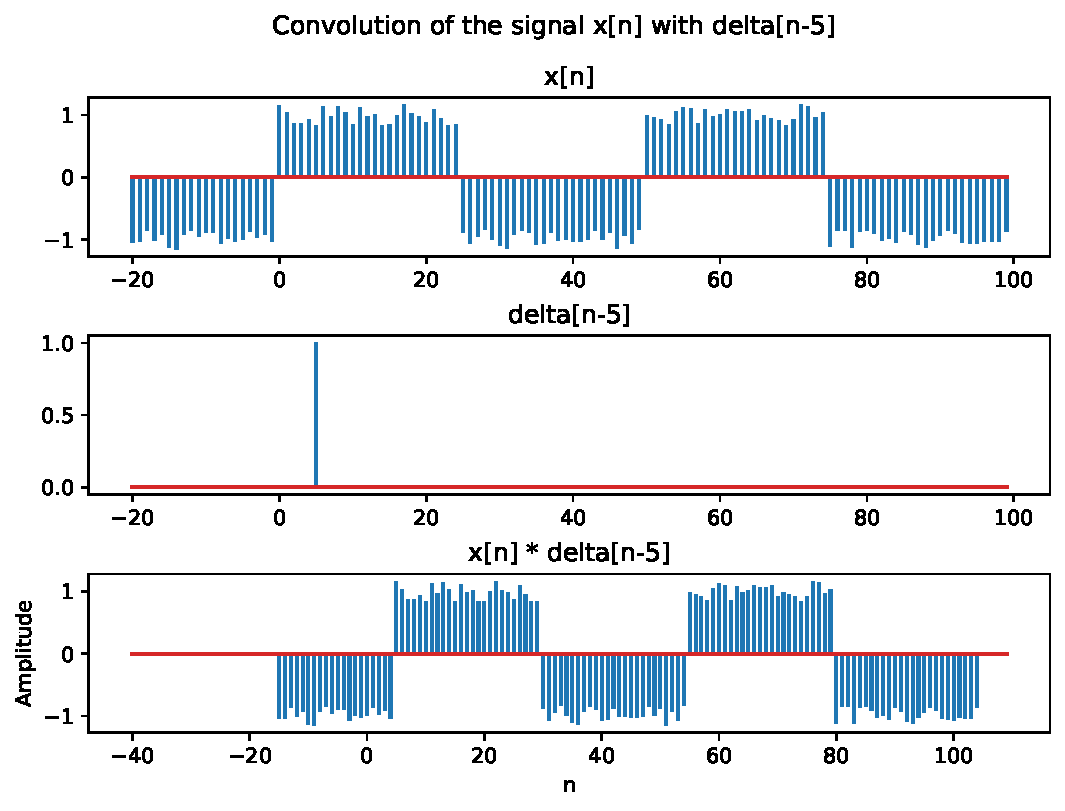
\includegraphics[width=1\textwidth]{q7/7a_convolution.pdf}
    \caption{Convolution of the signal with $\delta[n-5]$}
    \label{fig:figure2}
    \end{figure}

    
    \item %write the solution of q7b
    As we can see in the Figure 2,3,4, the N-Point Moving Average filter keeps the n values of our data and takes the average of them and equates them to our current position. In this way, it makes the signal smoother. So x[n] = (x[n] + x[n - 1] + ... + x[n - N + 1]) /N
    \begin{figure}[!htb]
    \centering
    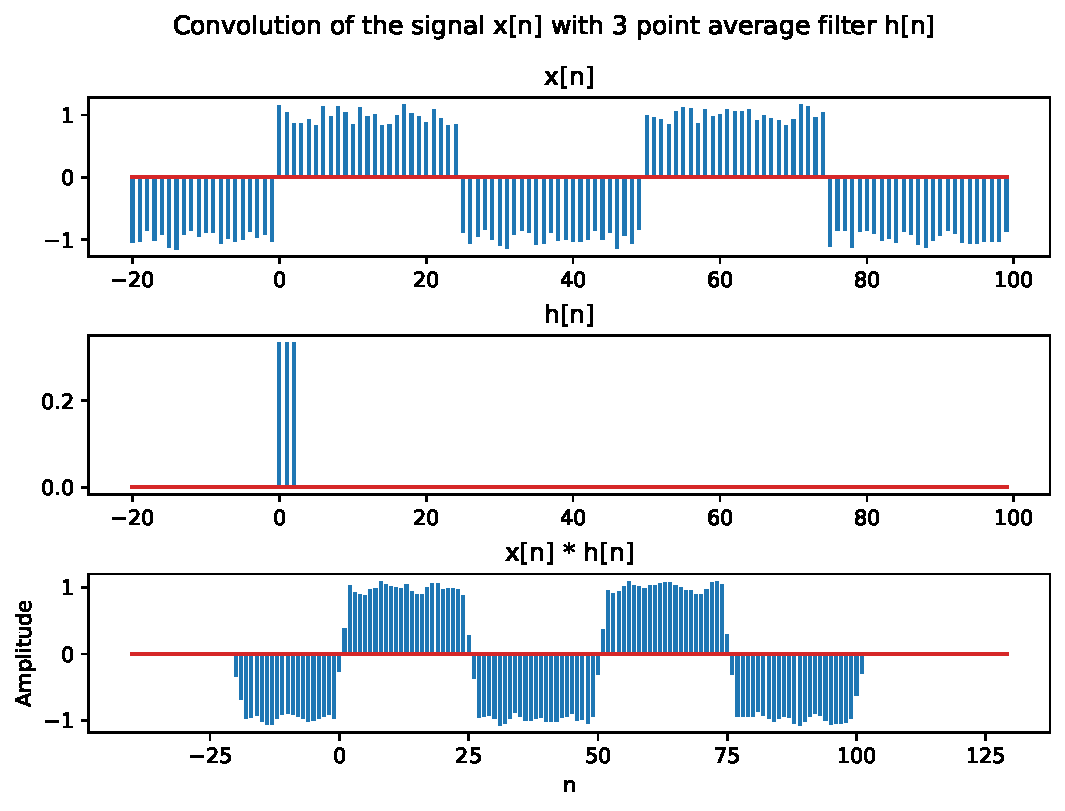
\includegraphics[width=1\textwidth]{q7/7b_convolution3.pdf}
    \caption{Convolution of the signal with 3-Point Moving Average Filter $h[n]$}
    \label{fig:figure2}
    \end{figure}
    
    \begin{figure}[!htb]
    \centering
    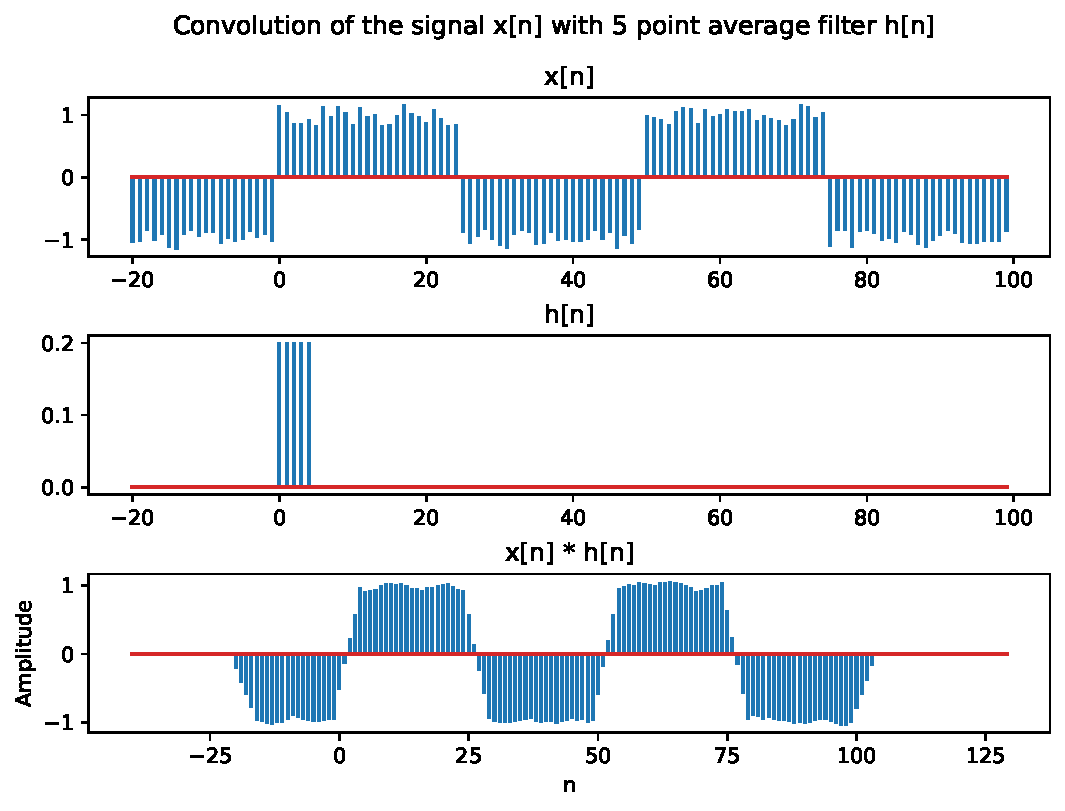
\includegraphics[width=1\textwidth]{q7/7b_convolution5.pdf}
    \caption{Convolution of the signal with 5-Point Moving Average Filter $h[n]$}
    \label{fig:figure2}
    \end{figure}
    
    \begin{figure}[!htb]
    \centering
    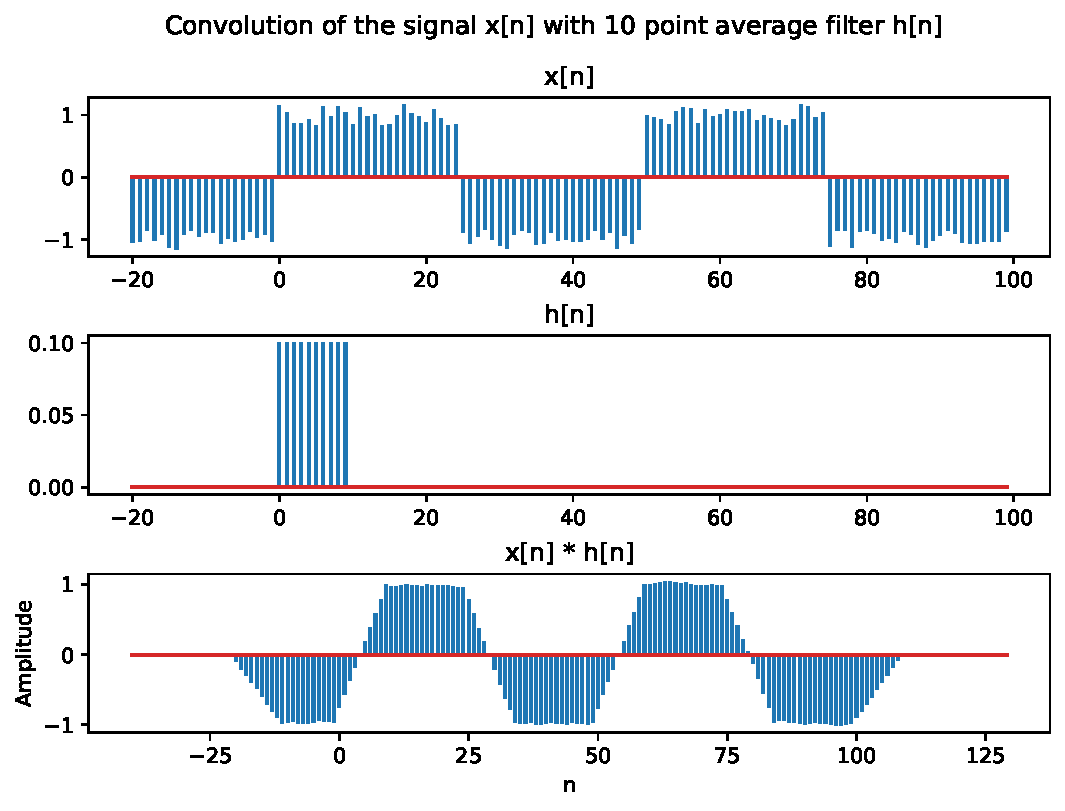
\includegraphics[width=1\textwidth]{q7/7b_convolution10.pdf}
    \caption{Convolution of the signal with 10-Point Moving Average Filter $h[n]$}
    \label{fig:figure2}
    \end{figure}
    
    \begin{figure}[!htb]
    \centering
    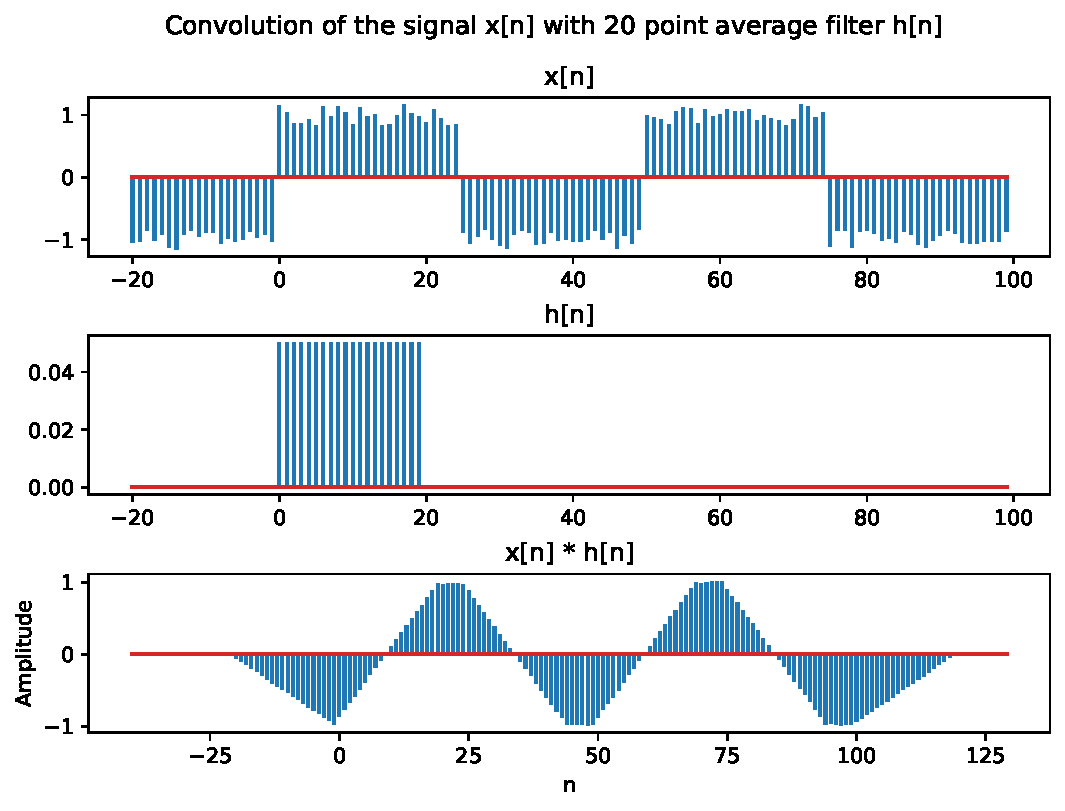
\includegraphics[width=1\textwidth]{q7/7b_convolution20.pdf}
    \caption{Convolution of the signal with 20-Point Moving Average Filter $h[n]$}
    \label{fig:figure2}
    \end{figure}
    \end{enumerate}    

\end{enumerate}


\end{document}
